\documentclass[10pt]{article}
\usepackage[a4paper,margin=20mm]{geometry}
\usepackage{amsmath,amssymb,amsthm,mathtools,booktabs}
\usepackage[T1]{fontenc}
\usepackage{xcolor,hyperref}
\usepackage{pgfplots}
\pgfplotsset{compat=1.18}
\hypersetup{colorlinks=true,linkcolor=blue,citecolor=blue,urlcolor=blue}
% Temporary reading theme: use \darkreadingfalse for printing.
\newif\ifdarkreading
\darkreadingtrue
\ifdarkreading
 \definecolor{readingbackground}{HTML}{202124}
 \definecolor{readingtext}{HTML}{E8EAED}
 \definecolor{readinglink}{HTML}{8AB4F8}
 \pagecolor{readingbackground}
 \AtBeginDocument{\color{readingtext}}
 \hypersetup{linkcolor=readinglink,citecolor=readinglink,urlcolor=readinglink}
\fi
\newcommand{\dd}{\,\mathrm d}
\newcommand{\Cl}{\operatorname{Cl}_2}
\newcommand{\Li}{\operatorname{Li}_2}
\newcommand{\EF}[2]{E_4\!\left(\begin{smallmatrix}#1\\#2\end{smallmatrix};u,\mathbf a\right)}
\newtheorem{theorem}{Theorem}
\setlength{\abovedisplayskip}{6pt}
\setlength{\belowdisplayskip}{6pt}
\title{A compact representation of the third-order Fock coefficient of helium}
\author{}
\date{}
% The native compiler checks the requested page budget, including references.
\newcounter{manuscriptpages}
\AddToHook{shipout/after}{\stepcounter{manuscriptpages}}
\AtEndDocument{\clearpage\ifnum\value{manuscriptpages}>5\relax
 \PackageError{PageBudget}{Exceeded 5-page budget; got \arabic{manuscriptpages}}{Adjust the layout.}\fi}
\begin{document}
\maketitle
\vspace{-1.5em}
\begin{abstract}
We express the third-order, nonlogarithmic Fock coefficient of a two-electron $S$-state as a finite combination of classical functions and elliptic polylogarithms.
Equivalent one-dimensional integrals provide a fast numerical evaluator.
An exact Python/SymPy--FLINT certificate verifies the angular recurrence; regularity establishes uniqueness.
Julia evaluates the formula and checks the full Schr\"odinger residual by automatic differentiation.
The appendix gives the quadrature-free form and discusses further simplification.
\end{abstract}

\section{Introduction}
Near the simultaneous electron--nucleus collision, the wavefunction has the Fock expansion
\begin{equation}
 \Psi=\sum_{k\ge0}R^k\sum_{p=0}^{\lfloor k/2\rfloor}(\log R)^p\psi_{k,p}(\alpha,\theta),
 \qquad R=\sqrt{r_1^2+r_2^2},\quad\alpha=2\arctan(r_2/r_1),\quad\psi_{0,0}=1.
\end{equation}
Here $\theta$ is the angle between the electron position vectors; the nucleus  has charge $Z$.
Liverts and Barnea obtained explicit component formulas and an angular Green representation~\cite{LB2015,LB2017}; Liverts evaluated its azimuthal integral in elliptic functions~\cite{L2021}.
Langner's thesis gives the full third-order coefficient as convergent double series~\cite{Langner2022}.
Our contribution is a compact evaluation of $\psi_{3,0}$, with no angular-mode sum, and a direct verification independent of the third-order starting series.

\section{The formula}
The formula holds for $0<\alpha,\theta<\pi$, with boundary values defined by continuity.
Let $a_{21}$ be the total coefficient of the harmonic $\sin\alpha\cos\theta$ in $\psi_{2,0}$, following Ref.~\cite{LK2024}.
Then
\begin{equation}\label{eq:answer}
\begin{aligned}
\psi_{3,0}={}&\mathcal D(\alpha,\theta;Z)
 +\frac{Z\sqrt{1+\sin\alpha}}{36}\bigl[E(4+\sin\alpha)-18a_{21}\sin\alpha\cos\theta\bigr]\\
 &+\frac{\sqrt{1-\sin\alpha\cos\theta}}{72}
 \bigl[6a_{21}-5E+(30a_{21}-E)\sin\alpha\cos\theta\bigr]\\
 &+F_{\rm a}\left(\cos\alpha,-\sqrt{\frac{1-\sin\alpha\cos\theta}{2}}\right)
 +F_{\rm a}\left(-\cos\alpha,-\sqrt{\frac{1-\sin\alpha\cos\theta}{2}}\right)\\
 &+F_{\rm r}\bigl(-\sin\alpha\cos\theta,-\cos(\alpha/2)\bigr)
 +F_{\rm r}\bigl(-\sin\alpha\cos\theta,-\sin(\alpha/2)\bigr),
\end{aligned}
\end{equation}
where $F_{\rm a}=c_0^{\rm a}N_0+c_2^{\rm a}N_2$ and $F_{\rm r}=c_0^{\rm r}N_0+c_2^{\rm r}N_2$.
For each pair $(b,y)$, set $\kappa=\sqrt{(1+b)/(1-b)}$ and $u=\min(1,\kappa)$.
Let $\mathbf a=\mathbf a(b,y)$ be the four roots of $t^4+\frac{4y^2-2}{1-b}t^2+\kappa^2$, ordered as in Appendix~\ref{app:finite}.
Thus $y$ enters through the branch-point argument of the standard elliptic polylogarithms $E_4$~\cite{BDDT}:
\begin{gather}
 \begin{aligned}
 N_0(b,y)=\frac{1}{\sqrt{\kappa(1-b)}}\Biggl[&\frac\pi2\EF{0}{0}
 -2\Im\EF{0,1}{0,i}\\
 &-\frac2\pi\Re\left\{\EF{0,1,1}{0,i,i}-\EF{0,1,1}{0,i,-i}
 -\EF{0,1,1}{0,i\kappa,i\kappa}+\EF{0,1,1}{0,i\kappa,-i\kappa}\right\}\Biggr].
 \end{aligned}\label{eq:moments}\\
 c_0^{\rm a}=-\frac{\sqrt2Z(9Zb^2-18Z-8b^2+8)}{576},\qquad
 c_2^{\rm a}=\frac{\sqrt2Z(b-1)(90Zy^2-45Z-18b-32y^2+16)}{288},\nonumber\\
 c_0^{\rm r}=\frac{Z^2(1-b^2)}{18},\qquad
 c_2^{\rm r}=\frac{2Z^2(b-1)(2y^2-1)}9.\nonumber
\end{gather}
All four parameter pairs have $y<0$ in the physical interior.
The finite $E_4$ expression for $N_2$ is given in \eqref{eq:N2E4}.
All $E_4$ values share the endpoint $u$ and branch-point vector $\mathbf a(b,y)$; conjugate pairing reduces $N_0$ to six values.
An alternative integral representation explains the subscripts:
\begin{equation}\label{eq:moment-integral}
 N_k(b,y)=\int_0^1 t^k\log\frac{1+t}{1-t}\,
 \frac{\widehat A(t;b,y)}{\sqrt{P(t;b,y)}}\,\dd t,\qquad k=0,2,
\end{equation}
where
\[
 P(t;b,y)=1+b+(2-4y^2)t^2+(1-b)t^4,\qquad
 \widehat A(t;b,y)=\frac2\pi\arctan\frac{\sqrt{P(t;b,y)}}{-2yt}.
\]
Only the weights $1$ and $t^2$ occur in the formula.
The dilogarithmic term $\mathcal D$ is specified below.

\subsection*{The dilogarithmic term}
In this term define $\beta=\arccos(\sin\alpha\cos\theta)$.
Here we use $\sigma=\sqrt{1+\sin\alpha}$, $\delta=\cos(\alpha/2)-\sin(\alpha/2)$ and $\eta=\sqrt{1+\sin\alpha\cos\theta}$.
Write $x=\alpha-\pi/2$, $p=\beta-\pi$, and $w_\varepsilon=(x+\varepsilon p)/4$ for $\varepsilon=\pm1$.
The functions required are
\begin{equation}
 \mathcal L(z)=z\log|2\sin z|+\tfrac12\Cl(2z),\qquad
 \mathcal T(z)=-z\log|2\cos z|+\tfrac12\Cl(\pi-2z),\quad
 \Cl(z)=\Im\Li(e^{iz}).
\end{equation}
Use the removable value $\mathcal L(0)=0$.
On the physical domain, $w_+\in[-\pi/4,0]$ and $w_-\in[0,\pi/4]$, so all displayed functions are finite.
Then
\begin{equation}\label{eq:dilogarithmic}
\begin{aligned}
 \mathcal D(\alpha,\theta;Z)={}&\sum_{\varepsilon=\pm1}\left[
 4\sum_{m=-1}^1K_m(\varepsilon\eta)\mathcal L(w_\varepsilon+m\pi/4)
 -4K_2(\varepsilon\eta)\mathcal T(w_\varepsilon)
 +e(\varepsilon\eta)\log|2\cos w_\varepsilon|\right]\\
 &+h\mathcal L\bigl((\pi-\beta)/2\bigr)
 +\frac{2Z^2}{9\pi}\Bigl[
 -\sin(\alpha/2)(4\cos\alpha+\sin\alpha\cos\theta)\mathcal L(\alpha/2)\\
 &\hspace{22mm}+\cos(\alpha/2)(4\cos\alpha-\sin\alpha\cos\theta)
 \mathcal L\bigl((\pi-\alpha)/2\bigr)\Bigr]\\
 &+q_{xx}x^2+q_x\,x+q_{pp}p^2+q_p\,p+\mathcal R.
\end{aligned}
\end{equation}
The identities $\sigma^2=1+\sin\alpha$ and $\sigma\delta=\cos\alpha$ simplify the coefficients.
For $m=-1,0,1,2$, respectively, let
\begin{equation}
 \delta_m=\sigma,\ \delta,\ -\sigma,\ -\delta.
\end{equation}
With $z=\pm\eta$, define
\begin{align}
 K_m(z)&=\frac{Z}{144\pi}\Bigl[-\delta_m\{9+8\sin\alpha\cos\theta+9(-1)^m\sin\alpha\}
 \nonumber\\ &\hspace{15mm}+6(-1)^m\sqrt{1-\sin\alpha\cos\theta}\cos\alpha-z(3+2\sin\alpha\cos\theta)\Bigr]\nonumber\\
 &\quad+\frac{5Z^2\sin\alpha\cos\theta(\delta_m+z)}{32\pi}
 +\frac{Z^2\delta\nu_m(z)}{36\pi},\label{eq:K}\\
 \nu_0(z)&=\nu_2(z)=-\sin\alpha\cos\theta-\sin\alpha,\qquad
 \nu_{\pm1}(z)=8-\sin\alpha\cos\theta+9\sin\alpha\mp8\sigma z,\nonumber\\
 e(z)&=\frac{Z\{7z\cos\alpha+\sigma(9\sin\alpha-8\sin\alpha\cos\theta-9)\}}{72}\nonumber\\ &\quad-\frac{Z\sqrt{1-\sin\alpha\cos\theta}(1+5\sin\alpha\cos\theta)}{36}\nonumber\\
 &\quad+\frac{Z^2\{137z\cos\alpha+\sigma(64\sin\alpha+154\sin\alpha\cos\theta-64)\}}{288},\nonumber\\
 h&=\frac{Z\eta\{(45Z-4)\sin\alpha\cos\theta-6\}}{36\pi},\nonumber\\ &
 q_{xx}=\frac{Z\sqrt{1-\sin\alpha\cos\theta}\{6+(45Z-4)\sin\alpha\cos\theta\}}{288\pi},\nonumber\\
 q_x&=\frac{Z\sqrt{1-\sin\alpha\cos\theta}\cos\alpha(28+9Z)}{576}-\frac{Z^2\delta\sin\alpha\cos\theta}{9\pi},\nonumber\\ &
 q_{pp}=\frac{Z^2\sigma(4\sin\alpha-\sin\alpha\cos\theta-4)}{36\pi},\nonumber\\
 q_p&=\frac{Z\eta(5\sin\alpha\cos\theta-1)}{36\pi}+\frac{Z^2\sigma\sqrt{1-\sin^2\alpha\cos^2\theta}}{18\pi}.\nonumber
\end{align}
Finally, with $G$ Catalan's constant and $\ell=\log2+4G/\pi$,
\begin{equation}\label{eq:remainder}
\begin{aligned}
 \mathcal R={}&\sqrt{1-\sin\alpha\cos\theta}\Biggl\{\frac{1+2\sin\alpha\cos\theta}{72}\\ &\hspace{10mm}
 +Z\left[\frac{(1+5\sin\alpha\cos\theta)\ell}{72}-\frac{\pi\sin\alpha\cos\theta}{36}
 \right.\\ &\hspace{20mm}\left.-\frac{15+91\sin\alpha\cos\theta}{144\pi}+\frac{4\sin\alpha+3+27\sin\alpha\cos\theta}{288}\right]\\
 &\hspace{26mm}+Z^2\left[\frac{5\pi\sin\alpha\cos\theta}{64}
 +\frac{71+375\sin\alpha-656\sin\alpha\cos\theta}{864}\right]\Biggr\}\\
 &+\sigma\Biggl\{\frac{Z(\sin\alpha-6+8\sin\alpha\cos\theta)}{72}-\frac{Z^3(2+5\sin\alpha)}{36}\\
 &\hspace{14mm}+Z^2\left[-\frac{\sin\alpha\cos\theta}{12}\left(\ell-\frac{53}{6\pi}\right)
 +\frac{\pi(4\sin\alpha+\sin\alpha\cos\theta-4)}{144}
 -\frac{503\sin\alpha-384\sin\alpha\cos\theta-325}{864}\right]\Biggr\}.
\end{aligned}
\end{equation}
These definitions require no fitted constants or implicit coefficient tables.
The parameters $Z,E,a_{21}$ may be varied without changing $N_0$ and $N_2$.

\section{Direct verification}
The accompanying Python/SymPy--FLINT code verifies exactly that our formula satisfies the third-order Fock recurrence.
Regularity and the absence of a regular homogeneous solution then establish uniqueness for the specified lower-order coefficients.
For this verification only, write $\xi=r_{12}/R=\sqrt{1-\sin\alpha\cos\theta}$.
The third-order Fock recurrence is
\begin{equation}\label{eq:recurrence}
 (\Lambda^2-21)\psi_{3,0}=10\psi_{3,1}-2V\psi_{2,0}+2E\psi_{1,0},\qquad
 V=\xi^{-1}-2Z\sigma/\sin\alpha.
\end{equation}
For $a=\cos\alpha$ and $v=\sin\alpha\cos\theta$, the operator and lower coefficients are
\begin{align}
 \Lambda^2&=-4\bigl[(1-a^2)\partial_a^2+(1-v^2)\partial_v^2-2av\partial_a\partial_v-3a\partial_a-3v\partial_v\bigr],\\
 \psi_{1,0}&=\xi/2-Z\sigma,\qquad
 \psi_{3,1}=\frac{Z(\pi-2)\xi(5\xi^2-6)}{36\pi}+\frac{Z^2(\pi-2)\sigma v}{6\pi},\nonumber\\
 \psi_{2,0}&=\frac{1-2E}{12}+Z(\chi-\sigma\xi/3)+Z^2(1/3+\tfrac12\sin\alpha)
 +\left[a_{21}-\frac{Z(\pi+4)}{9\pi}\right]v.\nonumber
\end{align}
Here $\chi$ is the regular solution with zero $K=2$ harmonic projection of
$(\Lambda^2-12)\chi=2\sigma/(3\xi\sin\alpha)-8(\pi-2)v/(3\pi)$; its known dilogarithmic formula~\cite{LB2015} is included in the certificate.

\begin{theorem}
Equation~\eqref{eq:answer} is the unique regular coefficient satisfying \eqref{eq:recurrence} for the specified lower-order coefficients.
\end{theorem}
\begin{proof}
For verification, use the integral representation \eqref{eq:moment-integral}.
Its equivalence to \eqref{eq:moments} follows from the elementary identity
$\int_0^1t\log((1+t)/(1-t))/(t^2+q^2)\,\dd t=\arctan^2(1/q)$ for $q>0$, followed by partial fractions, a reciprocal substitution and the shuffle reduction in Appendix~\ref{app:finite}; the full derivation accompanies the code.
For each integral weight $Q=c_0+c_2t^2$, its action has the form
\begin{equation}
 (\Lambda^2-21)\frac{Q\widehat A}{\sqrt P}
 =\partial_t\frac{H\widehat A}{\sqrt P}
 +\frac1\pi\left(\frac{d_1t}{1+t^2}+\frac{d_2t}{D}+\frac{d_3t}{D^2}\right),
 \quad D=1+b+(1-b)t^2,
\end{equation}
where $H$ is cubic in $t$.
The accompanying code constructs and checks these polynomial identities exactly.
Integration by parts, retaining the finite logarithmic endpoint contribution, leaves classical conic integrals and elementary terms, all explicitly evaluated in the certificate.
After $T=\tan(\alpha/4)$ and $U=\tan(\beta/4)$, every residual coefficient is rational.
Exact arithmetic gives zero separately in the eight sectors $1,Z,Z^2,Z^3,E,EZ,a_{21},Za_{21}$; no numerical samples enter this check.
The coefficient reductions use the rational-function field $\mathbb Q(\sqrt2,i)(T,U,\pi,G,\log2)$, treating $\pi,G,\log2$ as formal constants.
The input $\chi$ is the zero-$K=2$-projection dilogarithmic formula of Ref.~\cite{LB2015}, implemented in \path{inputs/round2/sym_H.py}, function \texttt{chi}, with harmonic shift $-(3\pi+10-16G)/(24\pi)$.

For regularity, $0\le\widehat A/\sqrt P\le1/\sqrt{P+4y^2t^2}\le1/(\sqrt2t)$ on the closed physical domain.
Since $\log((1+t)/(1-t))/t$ is integrable, the panels extend continuously and remain bounded.
The dilogarithmic terms are also bounded on their stated argument intervals.
The boundary $a^2+v^2=1$ lifts to a codimension-two circle on $S^3$.
Logarithmic cutoffs about this circle have gradient and Laplacian $L^1$ norms tending to zero, so boundedness extends the interior equation distributionally across it.
The source is $L^2$; elliptic regularity gives $H^2$.
Since $\Lambda^2=-4\Delta_{S^3}$ has eigenvalues $4n(n+2)\ne21$, the solution is unique.
\end{proof}

\section{Numerical evaluation}
The Julia package \texttt{TwoElectronFockExpansion.jl} combines $c_0N_0+c_2N_2$ into one adaptive quadrature per pair $(b,y)$.
The timings use equivalent elementary integrals with finite endpoints, rather than the special-function evaluator in Appendix~\ref{app:finite}.
Table~\ref{tab:timing} reports Float64 results at three interior points, with requested relative quadrature tolerance $10^{-12}$.
Times are medians of 101 evaluations after ten warm-up calls, excluding compilation, using one thread in Julia 1.13.1 on ARM64 macOS (CPU target \texttt{apple-m1}).
\begin{table}[h]
\centering
\begin{tabular}{rrrcc}\toprule
$a$ & $r_{12}/R$ & $\psi_{3,0}$ & absolute discrepancy & time ($\mu$s)\\\midrule
$0.30$ & $0.90$ & $-1.973118193998715$ & $7.23\times10^{-16}$ & $15$\\
$-0.27$ & $1.13$ & $-1.112107042879925$ & $6.46\times10^{-16}$ & $14$\\
$0.20$ & $1.00$ & $-1.143280767511434$ & $6.45\times10^{-16}$ & $15$\\\bottomrule
\end{tabular}
\caption{Julia quadrature evaluator compared with independently checked high-precision reference values.
The first row uses $(Z,E,a_{21})=(2,-2.9,0.123)$; the others use $(1.7,-2.2,0.31)$.}
\label{tab:timing}
\end{table}
Quadrature estimates exclude cancellation and roundoff in $\mathcal D$.
The current Julia implementation excludes exact collision endpoints, where separate limits or higher precision are needed.
Independently, conversion to the torus functions implemented in GiNaC 1.8.10~\cite{GiNaCEMP} gives moment errors below $1.5\times10^{-36}$ at three parameter pairs and a full-coefficient error of $1.04\times10^{-37}$ at the first tabulated point.

\paragraph{Residual of the truncated wavefunction.}
We also apply ForwardDiff to the full third-order expansion
$\Psi^{(3)}=1+R\psi_{1,0}+R^2(\psi_{2,0}+\log R\,\psi_{2,1})+R^3(\psi_{3,0}+\log R\,\psi_{3,1})$.
Its gradient and Hessian give $(H-E)\Psi^{(3)}$ directly, without substituting the Fock recurrence.
For $Z=2$, $E=-2.9037243770341195983\ldots$ and our ground-state estimate $a_{21}=0.47674787900$, Fig.~\ref{fig:full-residual} shows the residual tending to zero with $R$, consistently with $O(R^2\log R)$ at fixed interior angles.
The 192- and 256-bit calculations agree within $6.73\times10^{-52}$.
At $(\alpha,\theta)=(2.2,2.4)$, $(H-E)\Psi^{(3)}/R^2=16.1067+1.26173\log R+O(R\log R)$: cancellation near $R=2.86\times10^{-6}$ explains the dip, after which the scaled absolute residual grows again.

\begin{figure}[htbp]
\centering
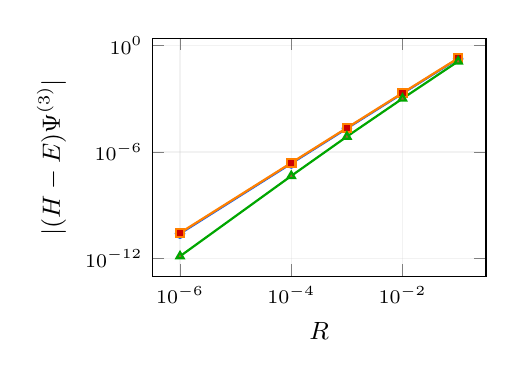
\begin{tikzpicture}
\begin{loglogaxis}[width=.48\textwidth,height=4.6cm,xlabel={$R$},ylabel={$|(H-E)\Psi^{(3)}|$},grid=major,grid style={opacity=.2},tick label style={font=\scriptsize},label style={font=\small},legend style={font=\scriptsize,draw=none,fill=none},legend pos=north west]
\addplot+[blue!65!cyan,mark=*,thick,mark size=1.5pt] coordinates {(1e-06,2.50238499673e-11) (0.0001,2.25124971376e-07) (0.001,2.12509305119e-05) (0.01,0.00199369064199) (0.1,0.181330510232)};
\addplot+[orange,mark=square*,thick,mark size=1.5pt] coordinates {(1e-06,2.74707364758e-11) (0.0001,2.43471012589e-07) (0.001,2.27817135944e-05) (0.01,0.00211847617407) (0.1,0.192954240123)};
\addplot+[green!65!black,mark=triangle*,thick,mark size=1.5pt] coordinates {(1e-06,1.32479067459e-12) (0.0001,4.48561409595e-08) (0.001,7.3890323515e-06) (0.01,0.00102673057946) (0.1,0.128163060598)};
\end{loglogaxis}
\end{tikzpicture}\hfill
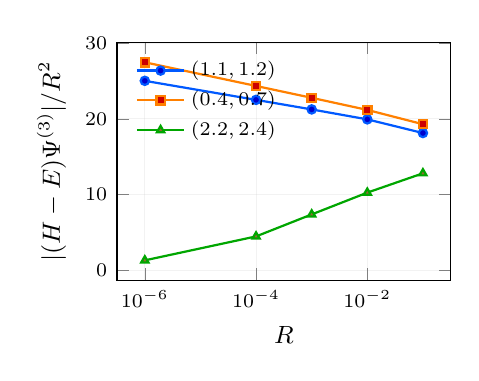
\begin{tikzpicture}
\begin{semilogxaxis}[width=.48\textwidth,height=4.6cm,xlabel={$R$},ylabel={$|(H-E)\Psi^{(3)}|/R^2$},grid=major,grid style={opacity=.2},tick label style={font=\scriptsize},label style={font=\small},legend style={font=\scriptsize,draw=none,fill=none},legend pos=north west]
\addplot+[blue!65!cyan,mark=*,thick,mark size=1.5pt] coordinates {(1e-06,25.0238499673) (0.0001,22.5124971376) (0.001,21.2509305119) (0.01,19.9369064199) (0.1,18.1330510232)};
\addlegendentry{$(1.1,1.2)$}
\addplot+[orange,mark=square*,thick,mark size=1.5pt] coordinates {(1e-06,27.4707364758) (0.0001,24.3471012589) (0.001,22.7817135944) (0.01,21.1847617407) (0.1,19.2954240123)};
\addlegendentry{$(0.4,0.7)$}
\addplot+[green!65!black,mark=triangle*,thick,mark size=1.5pt] coordinates {(1e-06,1.32479067459) (0.0001,4.48561409595) (0.001,7.3890323515) (0.01,10.2673057946) (0.1,12.8163060598)};
\addlegendentry{$(2.2,2.4)$}
\end{semilogxaxis}
\end{tikzpicture}
\caption{Full Schr\"odinger residual of the third-order Fock expansion, computed by automatic differentiation at the three $(\alpha,\theta)$ pairs in the legend.
The right panel divides out $R^2$ to display the remaining logarithmic dependence.}
\label{fig:full-residual}
\end{figure}

\appendix
\section{Finite evaluation and further simplification}\label{app:finite}
Use the standard $E_4$, $\omega_1$, $\eta_1$ and $Z_4$ conventions of Ref.~\cite{BDDT} on
\begin{equation}
 Y(t)^2=\frac{1+b+(4y^2-2)t^2+(1-b)t^4}{1-b},\qquad Y(0)=\kappa.
\end{equation}
Order the branch points as $(a_1,a_2,a_3,a_4)=(\zeta,\bar\zeta,-\zeta,-\bar\zeta)$, where $\zeta$ is the first-quadrant root.
The standard elliptic normalization is then $\tfrac12\sqrt{(a_1-a_3)(a_2-a_4)}=|\zeta|=\sqrt{\kappa}$.
Set $W=\sqrt{1-b}\,Y$ and $\gamma=(4y^2-2)/(6(1-b))+4\kappa\eta_1/\omega_1$, so that $Z_4'=(t^2+\gamma)/(\sqrt{\kappa}Y)$.
The remaining moment is
\begin{equation}\label{eq:N2E4}
\begin{aligned}
 N_2={}&\gamma N_0+\frac{\sqrt{\kappa}}{\sqrt{1-b}}\Biggl[\frac\pi2 Z_4(0)
 -\frac2\pi Z_4(u)\left\{\left(\frac\pi2-\arctan u\right)^2-\arctan^2(u/\kappa)\right\}\\
 &\quad+i\sum_{\varepsilon=\pm1}\varepsilon\EF{2}{\varepsilon i}
 -\frac1\pi\sum_{\varepsilon,\delta=\pm1}\varepsilon\delta
 \left\{\EF{2,1}{\varepsilon i,\delta i}-\EF{2,1}{\varepsilon i\kappa,\delta i\kappa}\right\}\Biggr]\\
 &+\frac{2}{i\pi\sqrt{1-b}}\sum_{\varepsilon=\pm1}\varepsilon
 \Biggl[\kappa\EF{-1,1}{\infty,\varepsilon i\kappa}+\EF{-1,1}{0,\varepsilon i\kappa}\\
 &\hspace{38mm}-\sqrt{\frac{1-y^2}{1-b}}\sum_{\delta=\pm1}\EF{-1,1}{\delta i\kappa,\varepsilon i\kappa}\Biggr]
 -\frac{2W(u)\arctan^2(u/\kappa)}{\pi(1-b)u}.
\end{aligned}
\end{equation}
Shuffle identities, $(W/t)'=(1-b)(t^2-\kappa^2/t^2)/W$ and integration by parts with $Z_4'$ give the formulas; exact checks verify the 51 unpaired coefficients and the conjugate pairing in \eqref{eq:moments}.
All endpoints are finite; at $b=0$ the length-three terms cancel.

Taylor continuation agrees with the previous evaluator within $5\times10^{-58}$ at the three tabulated points (65 digits).

Ordinary logarithms, dilogarithms and trilogarithms suffice when $\theta=0,\pi$; collinearity does not require $r_1=r_2$.
This paper establishes the representation and its recurrence; classification of further reductions and function-class obstructions is outside its scope.

\section*{Code and reproducibility}
The \path{verification/} directory contains the exact recurrence certificate, kernel derivations, benchmarks and reproduction instructions.
Within \path{verification/}, \path{compact_elliptic_moments/} and \path{ginac_validation/} contain the finite evaluator, $E_4$ checks and modular-transformation reproducer.

\section*{AI assistance}
OpenAI Codex and Anthropic Claude were used extensively for mathematical exploration, symbolic and numerical code, literature searches, and drafting and revision.
Agreement between AI systems was not treated as independent mathematical verification.
Responsibility for the manuscript and its claims rests with the human author.

{\small
\begin{thebibliography}{7}
\setlength{\itemsep}{0pt}
\setlength{\parskip}{0pt}
\bibitem{LB2015} E. Z. Liverts and N. Barnea, Angular Fock coefficients: Refinement and further development, \emph{Phys. Rev. A} \textbf{92}, 042512 (2015), \href{https://arxiv.org/abs/1505.02351}{arXiv:1505.02351}.
\bibitem{LB2017} E. Z. Liverts and N. Barnea, The Green's function approach to the Fock expansion calculations of two-electron atoms, \emph{J. Phys. A: Math. Theor.} \textbf{51}, 085204 (2018), \href{https://arxiv.org/abs/1705.09125}{arXiv:1705.09125}.
\bibitem{L2021} E. Z. Liverts, Co-spherical electronic configuration of the helium-like atomic systems, \emph{Ann. Phys.} \textbf{436}, 168669 (2022), \href{https://arxiv.org/abs/2106.11254}{arXiv:2106.11254}.
\bibitem{Langner2022} J. Langner, \emph{Towards an exact solution to the Schr\"odinger Equation of the Helium atom}, Ph.D. thesis, National Yang Ming Chiao Tung University (2022).
\bibitem{LK2024} E. Z. Liverts and R. Krivec, Two-Electron Atomic Systems---A Simple Method for Calculating the Ground State near the Nucleus: Some Applications, \emph{Atoms} \textbf{12}, 69 (2024), \href{https://doi.org/10.3390/atoms12120069}{doi:10.3390/atoms12120069}.
\bibitem{BDDT} J. Broedel, C. Duhr, F. Dulat and L. Tancredi, Elliptic polylogarithms and iterated integrals on elliptic curves. Part I: general formalism, \emph{JHEP} \textbf{05}, 093 (2018), \href{https://arxiv.org/abs/1712.07089}{arXiv:1712.07089}.
\bibitem{GiNaCEMP} C. Duhr, F. Lorkowski, R. Marzucca, S. Mauc and S. Weinzierl, Elliptic Multiple Polylogarithms with Arbitrary Arguments in GiNaC (2026), \href{https://arxiv.org/abs/2602.09956}{arXiv:2602.09956}.
\end{thebibliography}
}
\end{document}
